%%%%%%%%%%%%%%%%%%%%%%%%%%%%%% -*- Mode: Latex -*- %%%%%%%%%%%%%%%%%%%%%%%%%%%%
%% 04-21.tex -- IEEE Software Paper on Telemetry
%% Author          : Philip Johnson
%% Created On      : Mon Sep 23 11:52:28 2002
%% Last Modified By: Philip M. Johnson
%% Last Modified On: Mon Dec 06 10:14:54 2004
%% RCS: $Id$
%%%%%%%%%%%%%%%%%%%%%%%%%%%%%%%%%%%%%%%%%%%%%%%%%%%%%%%%%%%%%%%%%%%%%%%%%%%%%%%
%%   Copyright (C) 2002 Philip Johnson
%%%%%%%%%%%%%%%%%%%%%%%%%%%%%%%%%%%%%%%%%%%%%%%%%%%%%%%%%%%%%%%%%%%%%%%%%%%%%%%
%% 

%% Review: David Zubrow/SEI

\documentclass[11pt,twocolumn]{article} 
\input{/export/home/csdl/tex/psfig/psfig}
\usepackage{/export/home/csdl/tex/icse2003/latex8}
\usepackage{times}
%% A verbatim-like environment which allows font changes
%%\usepackage{alltt}
%% New LaTeX2e graphics support
\usepackage[final]{graphicx}
% uncomment the % away on next line to produce the final camera-ready version
% and uncomment the \thispagestyle{empty} following \maketitle
\pagestyle{empty}

\begin{document}

\title{ICSE Formal Demonstration Proposal: \\
      Hackystat: A framework for automated collection and analysis \\ 
      of software process and product measures}


\author{Philip M. Johnson \\
\em  Collaborative Software Development Laboratory \\
\em  Department of Information and Computer Sciences \\
\em  University of Hawai'i \\
\em  Honolulu, HI 96822 \\
\em  johnson@hawaii.edu}
\maketitle
\thispagestyle{empty}

\Section{Introduction}
\label{sec:intro}

It is conventional wisdom in the software engineering research community
that metrics can improve the effectiveness of project management.
Proponents of software metrics quote theorists and practitioners from
Galileo's ``What is not measurable, make measurable'' \cite{Finkelstein82}
to DeMarco's ``You can neither predict nor control what you cannot
measure'' \cite{DeMarco82}.  Software metrics range from internal product
attributes, such as size, complexity, and modularity, to external process
attributes, such as effort, productivity, testing quality, and reliability
\cite{Fenton97}.

Despite the potential of metrics in theory, effectively applying them
appears to be far from mainstream in practice. For example, a recent case
study of over 600 software professionals revealed that only 27\% viewed
metrics as ``very'' or ``extremely'' important to their software project
decision making process \cite{Kulik2003}. The study also revealed that cost
and schedule estimation was the only use of metrics attempted by a majority
of respondents.

In this formal demonstration, I will present Hackystat, a system for
automated collection and analysis of software product and process measures.
Hackystat differs from other approaches to software measurement technology
in one or more of the following ways:

\begin{itemize}

\item Hackystat uses sensors to unobtrusively collect data from development
environment tools; there is no chronic overhead on developers to collect
product and process data.

\item Hackystat is tool, environment, process, and application agnostic.
The architecture does not suppose a specific operating system platform, a
specific integrated development environment, a specific software process,
or specific application area.  A Hackystat system is configured from a set
of modules that determine what tools are supported, what data is collected,
and what analyses are run on this data.

\item Hackystat is intended to provide in-process project management support. Many traditional software
metrics approaches are based upon the "project repository" method, in which data from prior completed
projects are used to make predictions about or support control of a current project. In contrast,
Hackystat is designed to collect data from a current, ongoing project, and use that data as feedback
into the current project. 

\item Hackystat provides infrastructure for empirical experimentation.  For
those wishing to compare alternative approaches to development, or for
those wishing to do longitudinal studies over time, Hackystat can provide a
low-cost approach to gathering certain forms of project data.

\item Hackystat is open source and is available to the academic and
commercial software development community for no charge.

\end{itemize}

The design of Hackystat \cite{csdl2-02-07,csdl2-03-12} has resulted from of prior
research in our lab on software measurement, beginning with research into
data quality problems with the PSP \cite{csdl-98-04,csdl-98-11} and which
continued with the LEAP system for lightweight, empirical, anti-measurement
dysfunction, and portable software measurement
\cite{csdl-99-08,csdl2-00-03}.


Figure \ref{fig:architecture} illustrates the overall architecture of the
system. First, the project development environment must be instrumented by
installing Hackystat sensors, which developers attach to the various tools
such as their editor, build system, configuration management system, and so
forth. Once installed, the Hackystat sensors unobtrusively monitor
development activities and send process and product data to a centralized
web service.  Project members can log in to the web server to see the
collected raw data and run analyses that integrate and abstract the raw
sensor data streams into telemetry.  Hackystat also allows project members
to configure ``alerts'' that watch for specific conditions in the telemetry
stream and send email when these conditions occur.


\Section {Applications: Software Project Telemetry}

A major application of Hackystat has been the development of a new approach to
software measurement analysis called ``Software Project Telemetry''. We define
Software Project Telemetry as a style of software engineering process and product
collection and analysis  which satisfies
the following properties:

{\em Software project telemetry data is collected automatically by tools
   that unobtrusively monitor some form of state in the project
   development environment.}  In other words, the software developers are
   working in a ``remote or inaccessable location'' from the perspective of
   metrics collection activities. This contrasts with software metrics data
   that requires human intervention or developer effort to collect, such as
   PSP/TSP metrics \cite{Humphrey95}.
        
{\em Software project telemetry data consists of a stream of
   time-stamped events, where the time-stamp is significant for analysis.}
   Software project telemetry data is thus focused on evolutionary
   processes in development.  This contrasts, for example, with Cocomo
   \cite{Boehm81}, where the time at which the calibration data was
   collected about the project is not significant.

{\em Software project telemetry data is continuously and immediately 
available to both developers and managers.}  Telemetry data is not hidden
away in some obscure database guarded by the software quality improvement
group.  It is easily visible to all members of the project for 
interpretation. 

{\em Software project telemetry exhibits graceful degradation.}
While complete telemetry data provides the best support for project
management, the analyses should not be brittle: they should still provide
value even if sensor data occasionally ``drops out'' during the
project. Telemetry collection and analysis should provide decision-making
value even if these activities start midway through a project.
         
{\em Software project telemetry is used for in-process
   monitoring, control, and short-term prediction.} Telemetry analyses
   provide representations of current project state and how it is changing
   at the time scales of days, weeks, or months.  The simultaneous display
   of multiple project state values and how they change over the same time
   periods allow opportunistic analyses---the emergent knowledge that one
   state variable appears to co-vary with another in the context of the
   current project.


Software Project Telemetry enables a more incremental, distributed,
visible, and experiential approach to project decision-making. For example,
if one finds that complexity telemetry values are increasing, {\em and}
that defect density telemetry values are also increasing, then one could
try corrective action (such as simplification of overly complex modules)
and see if that results in a decrease in defect density telemetry
values. One can also monitor other telemetry data to see if such
simplification has unintended side-effects (such as performance
degradation).  Figure \ref{fig:telemetryreport} shows a simple telemetry 
report, and Figure \ref{fig:telemetrycontrolcenter} shows a ``Telemetry Control Center'' 
we designed and implemented for continuous display of telemetry data streams. 

In this research demonstration, I will present results from the use of 
telemetry data in both academic and industrial settings. 


\Section{Other applications}

We have also used Hackystat to support build process management for the
Mission Data System project at Jet Propulsion Lab, and to investigate Test
Driven Design development processes in laboratory settings. In my Research
Demonstration, I will show how Hackystat is used to support each of these
other more specialized applications. Since they are of less general
interest than Software Project Telemetry, I will devote less time in my
presentation to them.

\Section{Current Status}

Hackystat is an open source project with sources, binaries, and
documentation available at http://www.hackystat.org.  There is also a
public server available at http://hackystat.ics.hawaii.edu.  Hackystat has
been under development for approximately three years, and currently
consists of around 900 classes and 60,000 lines of code.  Sensors are
available for a variety of tools including Eclipse, Emacs, JBuilder, Jupiter, Jira, Visual
Studio, Ant, JUnit, JBlanket, CCCC, DependencyFinder, Harvest, LOCC,
Office, and CVS.  Hackystat development has been supported by funding from 
NASA, NSF, IBM, and Sun Microsystems.

\Section{Appendix: Format of the Demonstration}

The demonstration will begin with a short, ten minute presentation on the 
general problem of automated software engineering metrics collection and analysis 
and the basic trade-offs: the more you automate, the more restricted the kinds of
data you can collect, but the more you require manual data collection, the more
expensive the data is to collect and assure of its reliability.  

After this introduction, I will demonstrate the tool, and show data we have
collected from the past two years on the Hackystat project itself as well
as on smaller projects in software engineering classroom settings.  This
demo will provide participants with a sense for how Hackystat collects and
supports interpretation of Active time, code size, code complexity, unit
test results, test coverage results, build results, configuration
management commits and churn, code review data, and defect data.

In the third part of the presentation, I will discuss our research results
to date, ranging from software project telemetry to build management for the
Mission Data System group at JPL.

In the final part of the presentation, I will discuss the challenges we are
currently confronting with automated metrics collection, the lessons learned, 
organizational indicators for successful or unsuccessful adoption of Hackystat,
and our future plans.


\section{Appendix: Example Slides}

In addition to the figures appearing at the end of this proposal, we have an online guided tour at
http://csdl.ics.hawaii.edu/$\sim$johnson/docbook/ which provides more examples
of the kinds of slides that will appear in this Formal Demonstration.

\begin{figure*}[h]
  \centering
  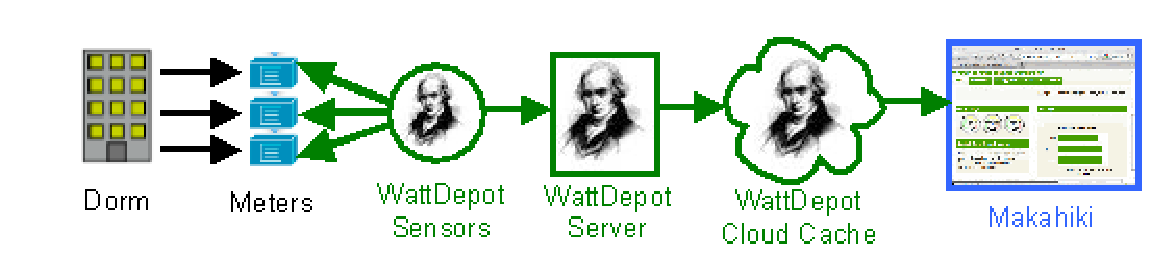
\includegraphics[width=0.75\textwidth]{architecture.eps}
  \caption{The basic architecture of Hackystat. Sensors are attached to
  tools directly invoked by developers (such as Eclipse or Emacs) as
  well as to tools implicitly manipulated by developers (such as CVS or 
  an automated build process using Ant).}
  \label{fig:architecture}
\end{figure*}


\begin{figure*}[h]
  \centering
  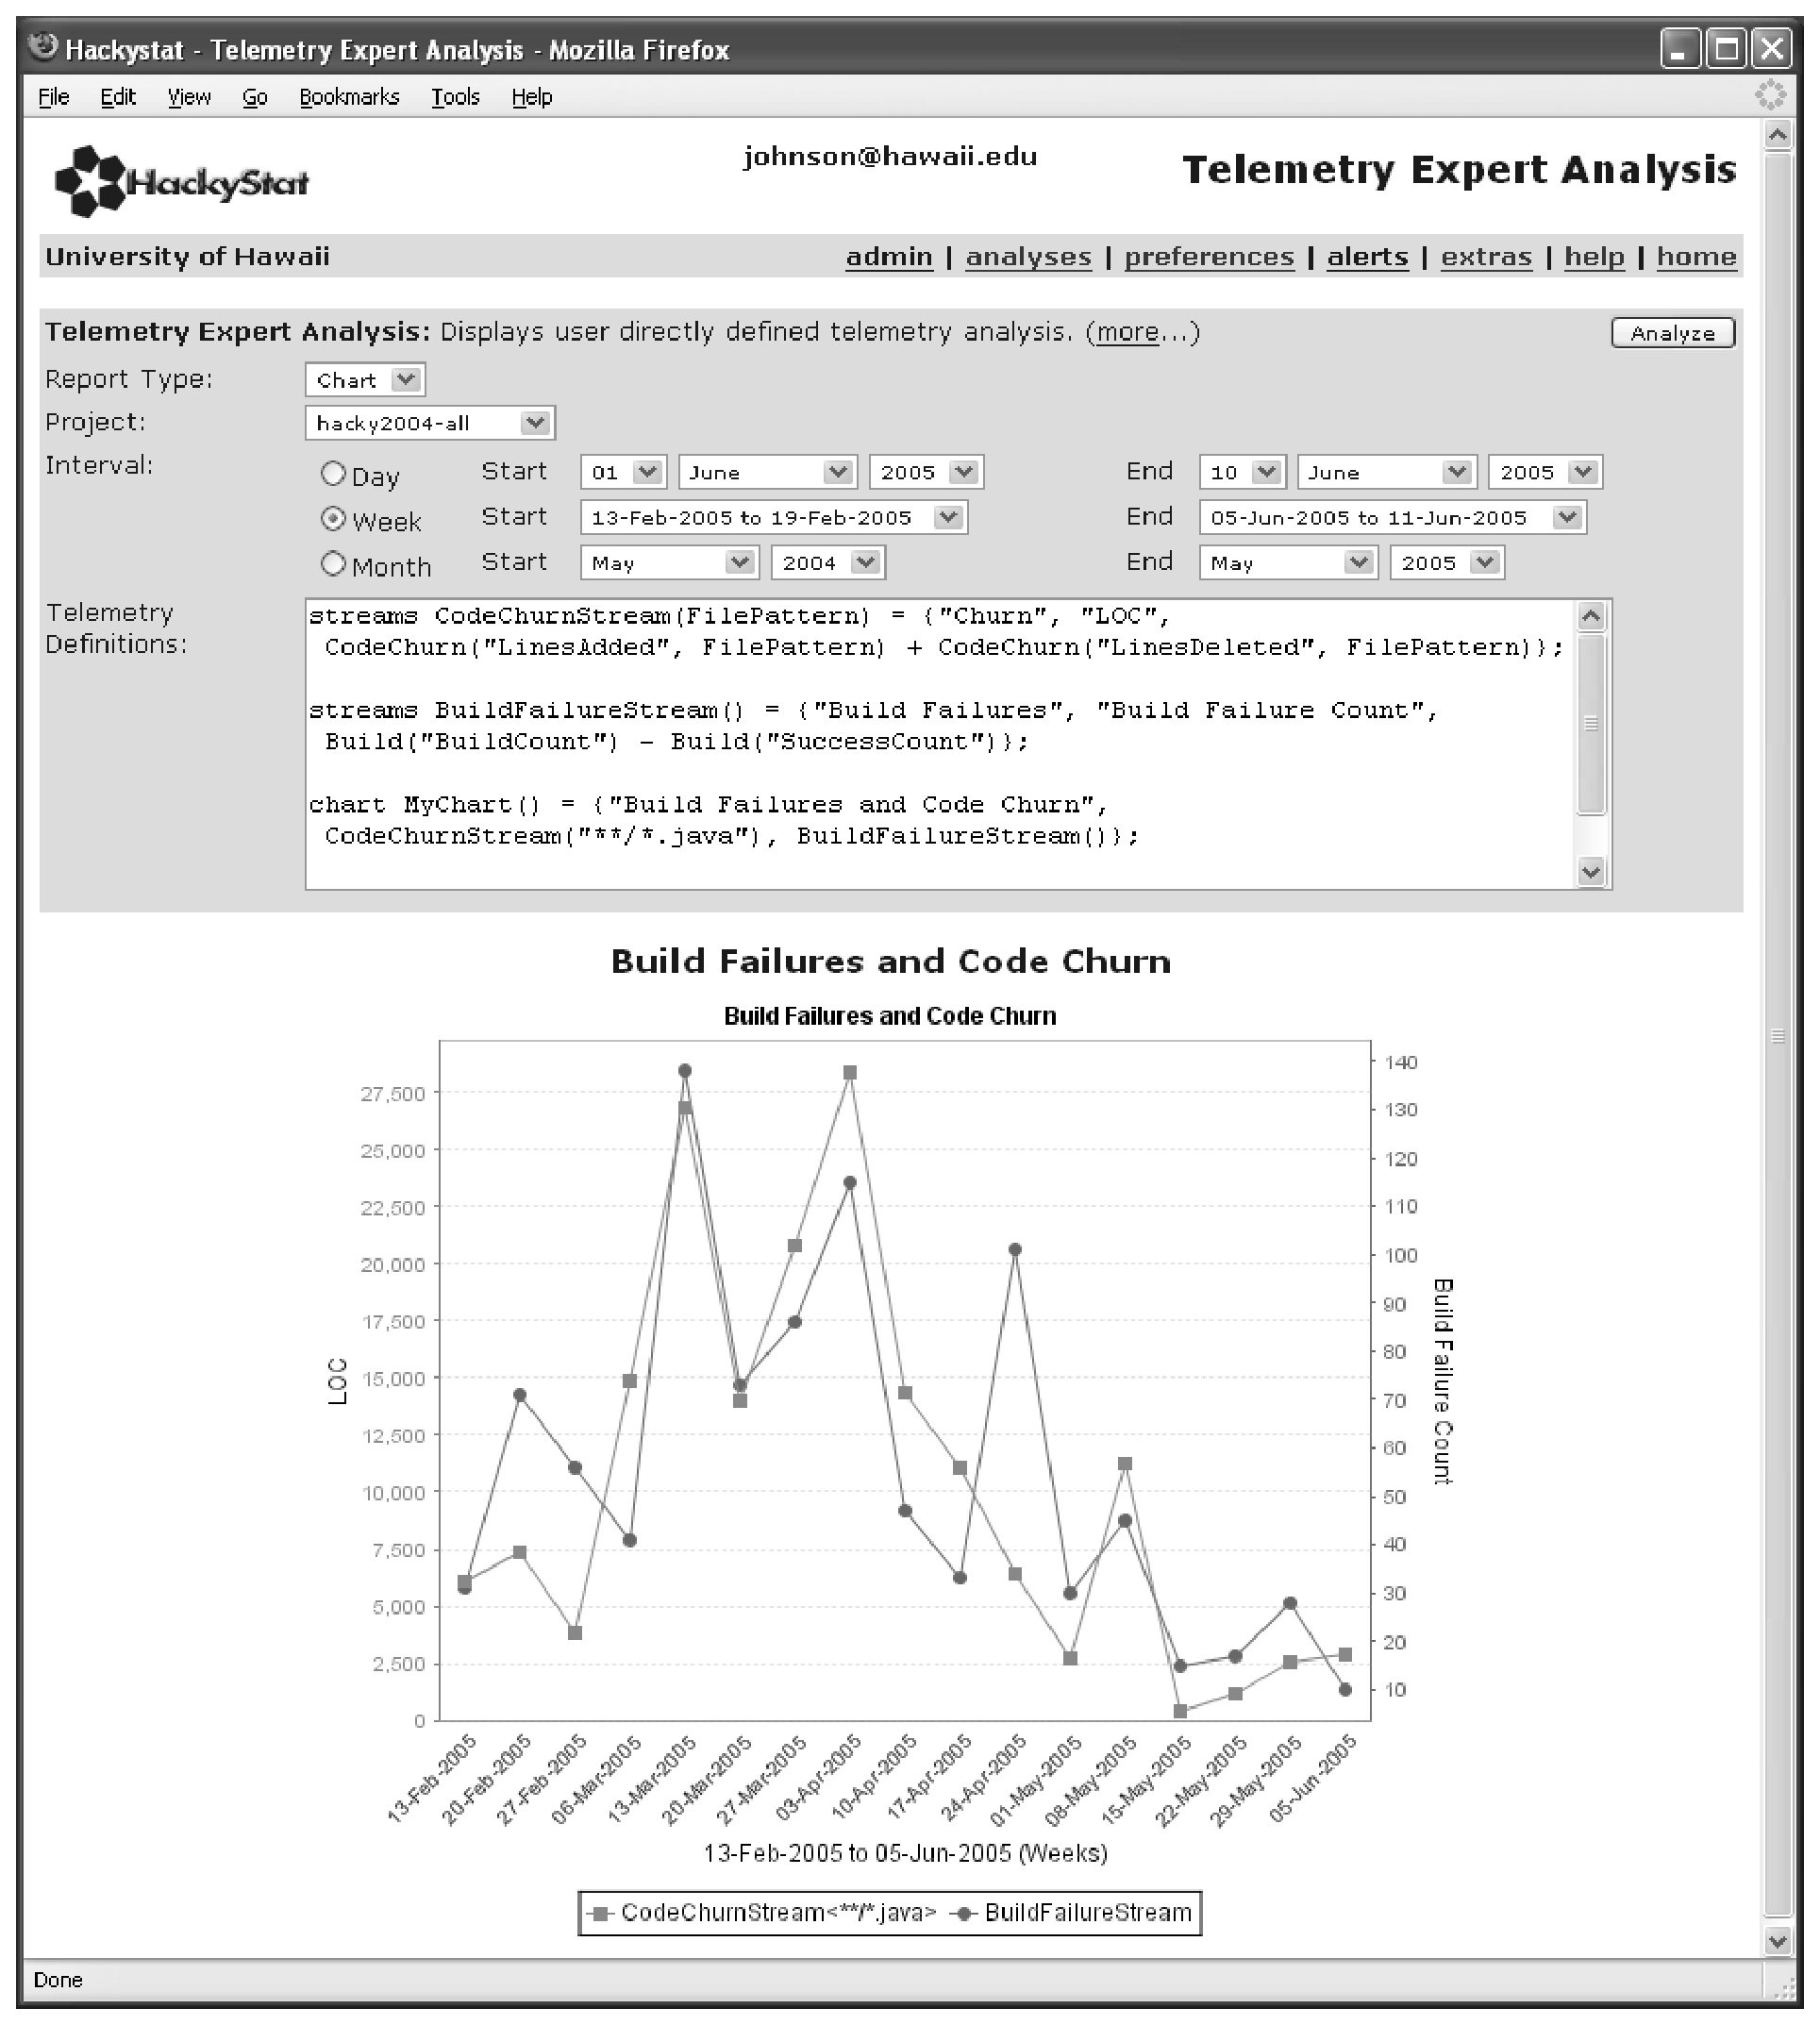
\includegraphics[width=0.75\textwidth]{BuildAndChurn.eps}
  \caption{A telemetry report that compares code churn (lines
  added and lines deleted) to build results (number of build attempts and
  number of failures.} 
  \label{fig:telemetryreport}
\end{figure*}

\begin{figure*}[h]
  \centering
  \includegraphics[width=0.75\textwidth]{Wall.eps}

  \caption{The Telemetry Control Center, showing one ``scene'' consisting
  of nine telemetry reports. The associated TelemetryViewer software 
  controls the TCC by automatically cycling
  through a set of scenes at a predefined interval. This 
  telemetry viewer is configured to show a dozen separate
  scenes, each displayed for two minutes.  }
  \label{fig:telemetrycontrolcenter}
\end{figure*}


\bibliographystyle{/export/home/csdl/tex/icse2003/latex8}
\bibliography{/export/home/csdl/techreports/04-11/04-11,/export/home/csdl/bib/csdl-trs,/export/home/csdl/bib/hackystat,/export/home/csdl/bib/psp}
\end{document}
 










